\documentclass[a4paper,11pt]{article}
\usepackage{geometry}
\geometry{
    left=20mm,
    right=20mm,
    top=22mm,
    bottom=22mm,
    footskip=12mm
}

\usepackage{fontspec}
\setmainfont{Times New Roman}
\setmonofont[Scale=0.9]{Consolas}

\usepackage[russian]{babel}
\usepackage{amsmath,amssymb,amsfonts}
\usepackage{graphicx}
\graphicspath{{../../src/}{../../src/figures/}{../src/}{../src/figures/}{../../}{../}{./}}
\usepackage{booktabs}
\usepackage{tabularx}
\usepackage{xcolor}
\usepackage{titlesec}
\usepackage{caption}
\usepackage{subcaption}
\usepackage{tcolorbox}
\usepackage{hyperref}

\hypersetup{
    colorlinks=true,
    linkcolor=blue!70!black,
    citecolor=blue!70!black,
    urlcolor=teal!70!black,
    pdftitle={Метод связанных волн (RCWA) для p-поляризации и полуаналитическое моделирование GIXRF},
    pdfauthor={Antigravity AI},
    pdfsubject={RCWA, TM polarization, Li factorization, Sherman equation, GIXRF, Rayleigh anomalies}
}

% Цветовая гамма
\definecolor{primary}{RGB}{16, 54, 98}
\definecolor{secondary}{RGB}{35, 95, 145}
\definecolor{accent}{RGB}{180, 50, 40}

\titleformat{\section}{\color{primary}\normalfont\Large\bfseries}{\thesection}{1em}{}
\titleformat{\subsection}{\color{secondary}\normalfont\large\bfseries}{\thesubsection}{1em}{}
\titleformat{\subsubsection}{\color{black}\normalfont\normalsize\bfseries}{\thesubsubsection}{1em}{}

% Стилизованные блоки
\newtcolorbox{mathbox}[1][Формула]{
    colback=blue!3!white,
    colframe=primary!80!black,
    fonttitle=\bfseries\color{white},
    title={#1},
    arc=2mm,
    boxrule=1pt,
    left=3mm,
    right=3mm,
    top=2mm,
    bottom=2mm
}

\newtcolorbox{remarkbox}[1][Замечание]{
    colback=gray!5!white,
    colframe=secondary!80!black,
    fonttitle=\bfseries\color{white},
    title={#1},
    arc=2mm,
    boxrule=0.8pt,
    left=3mm,
    right=3mm,
    top=2mm,
    bottom=2mm
}

\newtcolorbox{importantbox}[1][Важное положение]{
    colback=red!3!white,
    colframe=accent!90!black,
    fonttitle=\bfseries\color{white},
    title={#1},
    arc=2mm,
    boxrule=1pt,
    left=3mm,
    right=3mm,
    top=2mm,
    bottom=2mm
}

\begin{document}

\begin{titlepage}
    \centering
    \vspace*{1.5cm}
    {\Huge\bfseries\color{primary} Метод связанных волн (RCWA) для $p$ ($\pi$) поляризации и полуаналитическое моделирование рентгеновской флуоресценции (GIXRF)\par}
    \vspace{1cm}
    {\Large\itshape Строгий аналитический вывод от уравнений Максвелла и правил факторизации Ли до численного решения СЛАУ граничных условий и 2D угловых карт флуоресценции\par}
    \vspace{2cm}
    {\large\textbf{Автор:} Antigravity Advanced Pair Programming Assistant\par}
    \vfill
    {\large Октябрь 2026\par}
\end{titlepage}

\begin{abstract}
В настоящем фундаментальном руководстве представлен детальный математический и физический аппарат метода связанных волн (\textit{Rigorous Coupled-Wave Analysis}, RCWA / MBDDT) для \textbf{$p$ ($\pi$, TM) поляризации} рентгеновского излучения при скользящих углах падения (GIXD/GIXRF). В отличие от скалярного приближения для $s$-поляризации, где электрическое поле направлено вдоль однородной оси решетки, в $p$-поляризации вектор электрического поля лежит в плоскости дифракции и обладает двумя компонентами $(E_x, E_z)$, одна из которых испытывает разрыв на вертикальных границах наноструктур.

Документ охватывает 4 ключевых раздела:
\begin{enumerate}
    \item \textbf{Уравнения Максвелла, правила факторизации Ли и спектральная задача:} переход к скалярному магнитному полю $H_y$, математическое обоснование разрыва $E_x$ и непрерывности $D_x$, вывод обратного правила факторизации рядов Фурье Ли (Li, 1996), построение устойчивой матрицы взаимодействия $A^{(p)}$ через тёплицевы матрицы проницаемости $[\varepsilon]$ и обратной проницаемости $Z = [1/\varepsilon]$, спектральная задача на собственные значения.
    \item \textbf{Граничные условия, численно устойчивая СЛАУ и восстановление поля:} сшивка тангенциальных компонент $H_y$ и $E_x = -\frac{i}{\omega\varepsilon_0\varepsilon} \frac{\partial H_y}{\partial z}$, устранение экспоненциальной неустойчивости через привязку волн к точкам зарождения, вывод глобальной блочной СЛАУ $4D \times 4D$ и редуцированной системы $2D \times 2D$, алгоритм восстановления локальной плотности энергии поля $|E|^2 = |E_x|^2 + |E_z|^2$.
    \item \textbf{Полуаналитический расчет флуоресценции (GIXRF) для $p$-поляризации:} вывод из уравнения Шермана, точное разделение переменных для обеих векторных компонент поля, аналитическое интегрирование по латеральной координате (матрицы $U$ и $U^{(z)} = \mathcal{K}_x U \mathcal{K}_x$) и по глубине (матрицы $W$ и $W^{(x)}$), обобщенная полуаналитическая формула Николаева через произведение Адамара $F^{(p)}$.
    \item \textbf{Двумерные угловые карты флуоресценции $(\phi, \alpha_i)$ и кинематические линии Рэлея:} кинематический вывод уравнения дуг резонансов Рэлея-Вуда $\sin\phi = (\sin^2\alpha_i - \beta^2) / (2\beta\cos\alpha_i)$, поляризационные эффекты дифракции, влияние угла Брюстера и сопоставление топологии карт для $s$ и $p$ поляризаций.
\end{enumerate}
\end{abstract}

\newpage
\tableofcontents
\newpage

\section*{Введение и физическая постановка задачи}
\addcontentsline{toc}{section}{Введение и физическая постановка задачи}

Рентгеновская спектрометрия и рефлектометрия при скользящих углах падения (\textit{Grazing-Incidence X-ray Fluorescence}, GIXRF) являются ключевыми методами неразрушающей нанометровой метрологии периодических структур микро- и наноэлектроники \cite{soltwisch2018, nikolaev2020}. 

При скользящем падении рентгеновского пучка на периодическую нанорешетку электромагнитное поле разделяется на две ортогональные поляризационные моды:
\begin{itemize}
    \item \textbf{$s$-поляризация ($\sigma$, TE):} вектор электрического поля строго перпендикулярен плоскости падения ($\mathbf{E} = (0, E_y, 0)$). Вектор $\mathbf{E}$ направлен вдоль оси трансляционной инвариантности штрихов решетки, оставаясь тангенциальным ко всем границам раздела. Это позволяет использовать стандартное скалярное уравнение Гельмгольца и прямое правило Лорана для рядов Фурье.
    \item \textbf{$p$-поляризация ($\pi$, TM):} вектор магнитного поля перпендикулярен плоскости падения ($\mathbf{H} = (0, H_y, 0)$), а вектор электрического поля лежит в плоскости дифракции:
    \begin{equation}
        \mathbf{E} = \big(E_x(x, z), \, 0, \, E_z(x, z)\big).
    \end{equation}
\end{itemize}

В $p$-поляризации векторная природа уравнений Максвелла проявляется в полной мере:
\begin{enumerate}
    \item На вертикальных стенках наноштрихов ($x = \pm w/2$) нормальная компонента электрического поля $E_x$ испытывает \textbf{сильный скачок (разрыв первого рода)}, в то время как нормальная компонента электрической индукции $D_x = \varepsilon(x) E_x$ остается строго непрерывной.
    \item Прямое перемножение рядов Фурье (правило Лорана) в $p$-поляризации приводит к медленной сходимости $O(1/n)$ и осцилляциям Гиббса. Для устранения этой проблемы требуется применение \textbf{теоремы факторизации Ли (Li, 1996)} с использованием обратного правила (Inverse Rule).
    \item Выход характеристической флуоресценции возбуждается не магнитным, а \textbf{полным электрическим полем}:
    \begin{equation}
        |E(x, z)|^2 = |E_x(x, z)|^2 + |E_z(x, z)|^2.
    \end{equation}
    Поэтому полуаналитический метод интегрирования Николаева \cite{nikolaev2020} должен быть строго обобщен с учетом производных $\partial H_y / \partial z$ и $\partial H_y / \partial x$.
\end{enumerate}

Настоящий документ содержит полный, замкнутый теоретический вывод метода RCWA для $p$-поляризации, ориентированный на практическую реализацию в высокоточных алгоритмах численного моделирования.

\newpage
\section{Уравнения Максвелла, правила факторизации Ли и задача на собственные значения}

\subsection{Уравнения Максвелла и выбор базового скалярного поля}

Распространение монохроматического электромагнитного поля с гармонической временной зависимостью $e^{-i\omega t}$ описывается фундаментальной системой уравнений Максвелла:
\begin{align}
    \nabla \times \mathbf{E} &= i \omega \mu_0 \mathbf{H}, \label{eq:maxwell_curlE} \\
    \nabla \times \mathbf{H} &= -i \omega \varepsilon_0 \varepsilon(x) \mathbf{E}, \label{eq:maxwell_curlH} \\
    \nabla \cdot \big(\varepsilon(x) \mathbf{E}\big) &= 0, \label{eq:maxwell_divD} \\
    \nabla \cdot \mathbf{H} &= 0, \label{eq:maxwell_divB}
\end{align}
где $\varepsilon_0$ и $\mu_0$ — электрическая и магнитная постоянные вакуума, $K = \omega\sqrt{\varepsilon_0\mu_0} = \omega/c = 2\pi/\lambda$ — волновое число в вакууме, а $\varepsilon(x)$ — комплексная диэлектрическая проницаемость периодической решетки.

Для $p$ ($\pi$, TM) поляризации магнитное поле направлено вдоль оси $y$ (ортогонально плоскости дифракции $(x, z)$):
\begin{equation}
    \mathbf{H}(x, y, z) = \big(0, \, H_y(x, z), \, 0\big) \, e^{i K_y y},
\end{equation}
где для планарной дифракции ($\phi = 0$) компонента $K_y = 0$.

Раскроем оператор ротора магнитного поля в уравнении (\ref{eq:maxwell_curlH}):
\begin{equation}
    \nabla \times \mathbf{H} = \left( -\frac{\partial H_y}{\partial z}, \, 0, \, \frac{\partial H_y}{\partial x} \right).
\end{equation}
Приравнивая это к правой части $-i \omega \varepsilon_0 \varepsilon(x) \mathbf{E}$, немедленно выражаем обе компоненты электрического поля через производные единственной скалярной функции $H_y(x, z)$:
\begin{mathbox}[Связь компонент электрического поля с магнитным полем (p-поляризация)]
\begin{align}
    E_x(x, z) &= -\frac{i}{\omega \varepsilon_0 \varepsilon(x)} \frac{\partial H_y(x, z)}{\partial z}, \label{eq:Ex_from_Hy} \\[0.5em]
    E_z(x, z) &= \frac{i}{\omega \varepsilon_0 \varepsilon(x)} \frac{\partial H_y(x, z)}{\partial x}. \label{eq:Ez_from_Hy}
\end{align}
\end{mathbox}

Теперь подставим полученные выражения в закон индукции Фарадея (\ref{eq:maxwell_curlE}). Вектор $\nabla \times \mathbf{E}$ имеет единственную ненулевую $y$-компоненту:
\begin{equation}
    (\nabla \times \mathbf{E})_y = \frac{\partial E_x}{\partial z} - \frac{\partial E_z}{\partial x} = i \omega \mu_0 H_y.
\end{equation}
Подставляя соотношения (\ref{eq:Ex_from_Hy}) и (\ref{eq:Ez_from_Hy}):
\begin{equation}
    -\frac{i}{\omega \varepsilon_0} \left[ \frac{\partial}{\partial z} \left( \frac{1}{\varepsilon(x)} \frac{\partial H_y}{\partial z} \right) + \frac{\partial}{\partial x} \left( \frac{1}{\varepsilon(x)} \frac{\partial H_y}{\partial x} \right) \right] = i \omega \mu_0 H_y.
\end{equation}
Умножая обе части уравнения на $i \omega \varepsilon_0$ и учитывая, что $\omega^2 \varepsilon_0 \mu_0 = K^2$:
\begin{equation}
    \frac{\partial}{\partial z} \left( \frac{1}{\varepsilon(x)} \frac{\partial H_y}{\partial z} \right) + \frac{\partial}{\partial x} \left( \frac{1}{\varepsilon(x)} \frac{\partial H_y}{\partial x} \right) + K^2 H_y = 0.
\end{equation}
Поскольку профиль решетки в пределах слоя постоянен по глубине ($\varepsilon(x)$ зависит только от $x$ и не зависит от $z$), оператор $\partial / \partial z$ коммутирует с $1/\varepsilon(x)$:
\begin{mathbox}[Волновое дифференциальное уравнение второго порядка для $H_y$]
\begin{equation}
    \frac{1}{\varepsilon(x)} \frac{\partial^2 H_y}{\partial z^2} + \frac{\partial}{\partial x} \left( \frac{1}{\varepsilon(x)} \frac{\partial H_y}{\partial x} \right) + K^2 H_y = 0.
    \label{eq:wave_Hy_master}
\end{equation}
\end{mathbox}

\subsection{Теорема Флоке-Блоха и спектральное разложение поля}

В силу пространственной периодичности диэлектрической проницаемости $\varepsilon(x + d) = \varepsilon(x)$ с периодом $d$, согласно теореме Флоке-Блоха магнитное поле $H_y(x, z)$ раскладывается в дискретный ряд по пространственным гармоникам:
\begin{equation}
    H_y(x, z) = \sum_{h = -\infty}^{+\infty} H_h(z) \, e^{i k_{hx} x},
    \label{eq:bloch_Hy}
\end{equation}
где $k_{hx}$ — латеральный волновой вектор $h$-й пространственной гармоники:
\begin{equation}
    k_{hx} = K_x + \frac{2\pi h}{d} = K \cos\alpha_i \sin\phi + \frac{2\pi h}{d}.
\end{equation}
При численном расчете бесконечный ряд усекается до симметричного базиса из $D = 2n_{\max} + 1$ гармоник ($h \in [-n_{\max}, +n_{\max}]$). Определим вектор-столбец пространственных гармоник магнитного поля:
\begin{equation}
    \mathbf{H}(z) = \big[ H_{-n_{\max}}(z), \, \dots, \, H_0(z), \, \dots, \, H_{+n_{\max}}(z) \big]^T \in \mathbb{C}^D,
\end{equation}
и диагональный оператор латерального волнового вектора:
\begin{equation}
    K_x = \operatorname{diag}\big( k_{-n_{\max}, x}, \, \dots, \, k_{0x}, \, \dots, \, k_{+n_{\max}, x} \big).
\end{equation}

\subsection{Фундаментальные правила факторизации Фурье Ли (Li, 1996)}

Ключевая трудность классического метода связанных волн для TM-поляризации исторически заключалась в катастрофически медленной сходимости по числу гармоник. В 1996 году Ли (\textit{Lifeng Li}) \cite{li1996} доказал строгие математические теоремы о факторизации рядов Фурье для произведений разрывных периодических функций:

\begin{enumerate}
    \item \textbf{Прямое правило Лорана (Laurent's Rule):}
    Если хотя бы одна из двух перемножаемых периодических функций $f(x)$ и $g(x)$ является непрерывной во всех точках, коэффициенты Фурье их произведения $h(x) = f(x) g(x)$ сходятся к произведению тёплицевой матрицы $[f]$ и вектора коэффициентов $[g]$:
    \begin{equation}
        [h] = [f] [g].
    \end{equation}
    Это правило строго работает в $s$-поляризации, где поле $E_y(x)$ непрерывно.

    \item \textbf{Обратное правило Ли (Inverse Rule):}
    Пусть функции $f(x)$ и $g(x)$ имеют \textbf{одновременные скачки (одновременные разрывы первого рода)} в точках $x_j$, но их произведение $h(x) = f(x) g(x)$ является \textbf{непрерывной функцией}.
    В этом случае прямое правило Лорана $[f][g]$ терпит крах (сходимость падает до $O(1/n)$ из-за эффекта Гиббса). Точное преобразование требует факторизации через функцию с обратными значениями:
    \begin{equation}
        [h] = \left[ \frac{1}{f} \right]^{-1} [g].
        \label{eq:li_inverse_rule}
    \end{equation}
\end{enumerate}

Применим правила Ли к дифференциальному уравнению (\ref{eq:wave_Hy_master}):
\begin{itemize}
    \item Рассмотрим слагаемое $\frac{1}{\varepsilon(x)} \frac{\partial H_y}{\partial x}$. 
    Согласно (\ref{eq:Ez_from_Hy}), эта величина пропорциональна компоненте $E_z$. Но компонента $E_z$ направлена вдоль вертикальных стенок штриха ($x = \text{const}$) и, следовательно, является \textbf{тангенциальной} к этим границам! Из граничных условий электродинамики тангенциальное поле $E_z$ \textbf{строго непрерывно} при переходе через границу $x = \pm w/2$.
    Поскольку $1/\varepsilon(x)$ и $\partial H_y / \partial x$ разрывны, но их произведение непрерывно, по обратному правилу Ли (\ref{eq:li_inverse_rule}) получаем:
    \begin{equation}
        \left[ \frac{1}{\varepsilon(x)} \frac{\partial H_y}{\partial x} \right] = [\varepsilon]^{-1} \left[ \frac{\partial H_y}{\partial x} \right] = [\varepsilon]^{-1} (i K_x \mathbf{H}).
    \end{equation}
    \item Дифференцируя это выражение по $x$, применяем оператор $i K_x$:
    \begin{equation}
        \left[ \frac{\partial}{\partial x} \left( \frac{1}{\varepsilon(x)} \frac{\partial H_y}{\partial x} \right) \right] = (i K_x) [\varepsilon]^{-1} (i K_x \mathbf{H}) = - K_x [\varepsilon]^{-1} K_x \mathbf{H}.
    \end{equation}
    \item Теперь перепишем уравнение (\ref{eq:wave_Hy_master}) в виде:
    \begin{equation}
        \frac{\partial^2 H_y}{\partial z^2} = -\varepsilon(x) \left[ K^2 H_y + \frac{\partial}{\partial x} \left( \frac{1}{\varepsilon(x)} \frac{\partial H_y}{\partial x} \right) \right].
    \end{equation}
    Левая часть $\partial^2 H_y / \partial z^2$ непрерывна по $x$ (так как $H_y$ непрерывно). Следовательно, произведение $\varepsilon(x)$ на выражение в квадратных скобках также непрерывно. Применяя обратное правило Ли для умножения на $\varepsilon(x)$, мы заменяем оператор умножения на обратную матрицу от ряда Фурье величины $1/\varepsilon(x)$:
    \begin{equation}
        [\varepsilon]_{\text{eff}} = \left[ \frac{1}{\varepsilon} \right]^{-1} \equiv Z^{-1}, \quad \text{где } Z = \left[ \frac{1}{\varepsilon} \right].
    \end{equation}
\end{itemize}

Объединяя полученные результаты, получаем матричную дифференциальную систему:
\begin{equation}
    \frac{d^2 \mathbf{H}(z)}{dz^2} = - \Big[ Z^{-1} \big( K^2 I - K_x [\varepsilon]^{-1} K_x \big) - K_y^2 I \Big] \mathbf{H}(z).
\end{equation}

\begin{mathbox}[Матрица взаимодействия $A$ для p-поляризации (правило Ли 1996)]
\begin{equation}
    \frac{d^2 \mathbf{H}(z)}{dz^2} + A \mathbf{H}(z) = 0,
    \label{eq:matrix_diffeq_p}
\end{equation}
\begin{equation}
    A = Z^{-1} \Big( K^2 I - K_x [\varepsilon]^{-1} K_x \Big) - K_y^2 I, \quad \text{где } Z = \left[ \frac{1}{\varepsilon} \right].
    \label{eq:matrix_A_p_final}
\end{equation}
\end{mathbox}

\begin{remarkbox}[Сравнение матриц взаимодействия для s и p поляризаций]
В $s$-поляризации матрица взаимодействия имела вид $A^{(s)} = K^2 [\chi] + (K^2 I - K_x^2) = K^2 [\varepsilon] - K_x^2$. 
В $p$-поляризации в силу некоммутативности разрывных операторов матрица $A^{(p)} = Z^{-1} (K^2 I - K_x [\varepsilon]^{-1} K_x)$ содержит сразу две различные тёплицевы матрицы: матрицу самой проницаемости $[\varepsilon]$ и матрицу обратной проницаемости $Z = [1/\varepsilon]$. 
В рентгеновском диапазоне, где $\varepsilon = 1 + \chi$ с $|\chi| \ll 1$, матрицы $Z^{-1}$ и $[\varepsilon]$ отличаются на величину $O(\chi^2)$, однако учет правила Ли строго необходим для устранения высокочастотных артефактов на краях штрихов.
\end{remarkbox}

\subsection{Аналитические коэффициенты Фурье для ламеллярной решетки}

Для прямоугольного профиля штриха с шириной $w$ и периодом $d$ (коэффициент заполнения $\Gamma = w/d$) функции $\varepsilon(x)$ и $\eta(x) \equiv 1/\varepsilon(x)$ являются кусочно-постоянными:
\begin{equation}
    \varepsilon(x) = \begin{cases}
        \varepsilon_1, & |x| \le w/2 \text{ (штрих)}, \\
        \varepsilon_b, & w/2 < |x| \le d/2 \text{ (окружающая среда / вакуум, $\varepsilon_b = 1$)},
    \end{cases}
\end{equation}
\begin{equation}
    \eta(x) = \frac{1}{\varepsilon(x)} = \begin{cases}
        1/\varepsilon_1, & |x| \le w/2, \\
        1/\varepsilon_b, & w/2 < |x| \le d/2.
    \end{cases}
\end{equation}

Коэффициенты Фурье обеих функций вычисляются строго аналитически:
\begin{mathbox}[Коэффициенты Фурье диэлектрической проницаемости и обратной проницаемости]
\begin{align}
    \varepsilon_m &= (\varepsilon_1 - \varepsilon_b) \, \Gamma \, \operatorname{sinc}(m \Gamma) + \varepsilon_b \, \delta_{m, 0}, \label{eq:fourier_eps} \\[0.5em]
    \eta_m &= \left( \frac{1}{\varepsilon_1} - \frac{1}{\varepsilon_b} \right) \Gamma \, \operatorname{sinc}(m \Gamma) + \frac{1}{\varepsilon_b} \, \delta_{m, 0}, \label{eq:fourier_eta}
\end{align}
\end{mathbox}
где нормированная кардинальная функция синуса определена как $\operatorname{sinc}(\xi) = \frac{\sin(\pi \xi)}{\pi \xi}$ при $\xi \ne 0$ и $\operatorname{sinc}(0) = 1$.

Тёплицевы матрицы размера $D \times D$ формируются из коэффициентов разности индексов:
\begin{equation}
    [\varepsilon]_{gh} = \varepsilon_{g - h}, \quad Z_{gh} = \left[\frac{1}{\varepsilon}\right]_{gh} = \eta_{g - h}, \quad (g, h \in [-n_{\max}, +n_{\max}]).
\end{equation}

\subsection{Решение спектральной задачи на собственные значения}

Ищем решение векторной системы дифференциальных уравнений (\ref{eq:matrix_diffeq_p}) в виде элементарных собственных мод:
\begin{equation}
    \mathbf{H}(z) = \mathbf{E} \, e^{\pm i k_z z},
\end{equation}
где $\mathbf{E} = [E_{-n_{\max}}, \dots, E_0, \dots, E_{+n_{\max}}]^T$ — постоянный собственный вектор амплитуд гармоник, а $k_z$ — вертикальное волновое число моды.

Подставляя анзац в (\ref{eq:matrix_diffeq_p}):
\begin{equation}
    -k_z^2 \, \mathbf{E} \, e^{\pm i k_z z} + A \mathbf{E} \, e^{\pm i k_z z} = 0.
\end{equation}
Сокращая на скалярный ненулевой множитель $e^{\pm i k_z z}$, приходим к классической \textbf{алгебраической задаче на собственные значения и собственные векторы матрицы $A$}:

\begin{mathbox}[Спектральная задача для матрицы взаимодействия p-поляризации]
\begin{equation}
    A \mathbf{E}_n = k_{zn}^2 \mathbf{E}_n, \quad n = 1, \dots, D.
    \label{eq:eigenvalue_p}
\end{equation}
\end{mathbox}

\paragraph{Физический смысл матрицы собственных векторов $E$:}
Диагонализация матрицы $A$ дает $D$ собственных значений $\lambda_n = k_{zn}^2$ и $D$ соответствующих им собственных векторов $\mathbf{E}_n$. Объединяя столбцы $\mathbf{E}_n$, формируем модовую матрицу $E$:
\begin{equation}
    E = \big[ \mathbf{E}_1, \, \mathbf{E}_2, \, \dots, \, \mathbf{E}_D \big] \in \mathbb{C}^{D \times D}.
\end{equation}
Элемент $E_{hn} = (\mathbf{E}_n)_h$ представляет собой \textbf{амплитудный вес $h$-й пространственной гармоники $e^{i k_{hx} x}$ в $n$-й собственной моде решетки}:
\begin{equation}
    \psi_n(x, y, z) = e^{i K_y y} \left( \sum_{h=-n_{\max}}^{+n_{\max}} E_{hn} \, e^{i k_{hx} x} \right) e^{\pm i k_{zn} z}.
\end{equation}

Для обеспечения физического затухания поля в поглощающих средах комплексный корень $k_{zn} = \sqrt{k_{zn}^2}$ выбирается с положительными вещественной и мнимой частями:
\begin{equation}
    \operatorname{Re}(k_{zn}) \ge 0, \quad \operatorname{Im}(k_{zn}) \ge 0.
\end{equation}

\newpage
\section{Граничные условия, численно устойчивое решение и восстановление полей}

\subsection{Представление полей во всех областях пространства}

Рассмотрим трехслойную оптическую систему:
\begin{enumerate}
    \item \textbf{Верхнее полупространство ($z \le 0$):} вакуум ($\varepsilon_{\text{vac}} = 1$). Поле представляет собой суперпозицию падающей плоской волны единичной амплитуды и спектра отраженных дифракционных гармоник (с общим множителем $e^{i K_y y}$):
    \begin{equation}
        H_y^{\text{vac}}(x, y, z) = e^{i K_y y} \left[ e^{i K_x x} e^{i K_z z} + \sum_{h=-n_{\max}}^{+n_{\max}} R_h^{\text{vac}} \, e^{i k_{hx} x} e^{-i \kappa_{hz}^{\text{vac}} z} \right],
        \label{eq:Hy_vac}
    \end{equation}
    где вертикальное волновое число в вакууме в конической геометрии равно $\kappa_{hz}^{\text{vac}} = \sqrt{K^2 - K_y^2 - k_{hx}^2}$ с $\operatorname{Im}(\kappa_{hz}^{\text{vac}}) \ge 0$.
    \item \textbf{Слой наноструктуры ($0 \le z \le t$):} периодическая решетка. Поле представляется в виде устойчивой факторизации встречных собственных мод:
    \begin{equation}
        H_y^{\text{lay}}(x, y, z) = e^{i K_y y} \sum_{h} e^{i k_{hx} x} \sum_{n=1}^D E_{hn} \left[ T_n^{\text{lay}} \, e^{i k_{zn} z} + R_n^{\text{lay}} \, e^{-i k_{zn}(z - t)} \right],
        \label{eq:Hy_lay}
    \end{equation}
    где модовые амплитуды $T_n^{\text{lay}}$ привязаны к верхней границе $z = 0$, а $R_n^{\text{lay}}$ — к нижней границе $z = t$, что гарантирует экспоненциальную устойчивость.
    \item \textbf{Нижнее полупространство ($z \ge t$):} однородная подложка ($\varepsilon_{\text{sub}}$). Поле содержит только прошедшие волны, затухающие вглубь подложки:
    \begin{equation}
        H_y^{\text{sub}}(x, y, z) = e^{i K_y y} \sum_{h=-n_{\max}}^{+n_{\max}} T_h^{\text{sub}} \, e^{i k_{hx} x} e^{i \kappa_{hz}^{\text{sub}} (z - t)},
        \label{eq:Hy_sub}
    \end{equation}
    где $\kappa_{hz}^{\text{sub}} = \sqrt{\varepsilon_{\text{sub}} K^2 - K_y^2 - k_{hx}^2}$ с $\operatorname{Im}(\kappa_{hz}^{\text{sub}}) \ge 0$.
\end{enumerate}

\subsection{Электромагнитные граничные условия для p-поляризации}

На горизонтальных границах раздела $z = 0$ и $z = t$ электродинамические граничные условия требуют непрерывности тангенциальных компонент:
\begin{enumerate}
    \item Непрерывность тангенциального магнитного поля:
    \begin{equation}
        H_y(x, z^-) = H_y(x, z^+).
    \end{equation}
    \item Непрерывность тангенциального электрического поля $E_x$:
    Согласно уравнению (\ref{eq:Ex_from_Hy}), $E_x = -\frac{i}{\omega\varepsilon_0\varepsilon(x)} \frac{\partial H_y}{\partial z}$. Следовательно, непрерывной обязана быть величина:
    \begin{equation}
        \frac{1}{\varepsilon(x)} \frac{\partial H_y(x, z)}{\partial z} \quad \text{непрерывна при переходе через границы $z = 0$ и $z = t$!}
    \end{equation}
\end{enumerate}

\subsection{Пошаговый вывод блочной СЛАУ граничных условий}

Преобразуем граничные условия в векторно-матричный вид по дифракционным порядкам $h$:

\paragraph{1. Непрерывность $H_y$ на верхней границе ($z = 0$):}
Полагая $z = 0$ в уравнениях (\ref{eq:Hy_vac}) и (\ref{eq:Hy_lay}):
\begin{equation}
    \delta_{h, 0} + R_h^{\text{vac}} = \sum_{n=1}^D E_{hn} T_n^{\text{lay}} + \sum_{n=1}^D E_{hn} e^{i k_{zn} t} R_n^{\text{lay}}.
\end{equation}
Вводя диагональную матрицу фазовых множителей толщины $q = \operatorname{diag}\big(e^{i k_{zn} t}\big)$:
\begin{equation}
    - R^{\text{vac}} + E T^{\text{lay}} + E q R^{\text{lay}} = \boldsymbol{\delta}_0,
    \label{eq:bc1_p}
\end{equation}
где $\boldsymbol{\delta}_0 = [0, \dots, 0, 1, 0, \dots, 0]^T$ — единичный вектор возбуждения нулевого порядка.

\paragraph{2. Непрерывность $E_x \propto \frac{1}{\varepsilon} \frac{\partial H_y}{\partial z}$ на верхней границе ($z = 0$):}
\begin{itemize}
    \item В вакууме $\varepsilon_{\text{vac}} = 1$:
    \begin{equation}
        \left.\frac{1}{\varepsilon_{\text{vac}}} \frac{\partial H_y^{\text{vac}}}{\partial z}\right|_{z=0} = i K_z e^{i K_x x} - \sum_h i \kappa_{hz}^{\text{vac}} R_h^{\text{vac}} e^{i k_{hx} x}.
    \end{equation}
    \item В слое решетки производная равна:
    \begin{equation}
        \left.\frac{\partial H_y^{\text{lay}}}{\partial z}\right|_{z=0} = \sum_h e^{i k_{hx} x} \sum_n E_{hn} \big( i k_{zn} T_n^{\text{lay}} - i k_{zn} q_n R_n^{\text{lay}} \big).
    \end{equation}
    Поскольку величина $\partial H_y^{\text{lay}} / \partial z$ умножается на $1/\varepsilon(x)$, в силу взаимной гладкости поля вдоль границы $z = 0$ умножение в спектральном пространстве задается тёплицевой матрицей обратной проницаемости $Z = [1/\varepsilon]$:
    \begin{equation}
        \left[ \frac{1}{\varepsilon(x)} \left.\frac{\partial H_y^{\text{lay}}}{\partial z}\right|_{z=0} \right] = i \, Z \, E \, \mathcal{K} \, T^{\text{lay}} - i \, Z \, E \, \mathcal{K} \, q \, R^{\text{lay}},
    \end{equation}
    где $\mathcal{K} = \operatorname{diag}(k_{zn})$ — диагональная матрица вертикальных волновых чисел мод в слое.
\end{itemize}
Сокращая на мнимую единицу $i$ и вводя диагональный оператор $\mathcal{K}^{\text{vac}} = \operatorname{diag}(\kappa_{hz}^{\text{vac}})$:
\begin{equation}
    \mathcal{K}^{\text{vac}} R^{\text{vac}} + Z E \mathcal{K} T^{\text{lay}} - Z E \mathcal{K} q R^{\text{lay}} = \kappa_{0z}^{\text{vac}} \boldsymbol{\delta}_0.
    \label{eq:bc2_p}
\end{equation}

\paragraph{3. Непрерывность $H_y$ на нижней границе ($z = t$):}
Полагая $z = t$ в уравнениях (\ref{eq:Hy_lay}) и (\ref{eq:Hy_sub}):
\begin{equation}
    \sum_n E_{hn} q_n T_n^{\text{lay}} + \sum_n E_{hn} R_n^{\text{lay}} = T_h^{\text{sub}},
\end{equation}
что в векторно-матричной форме дает:
\begin{equation}
    E q T^{\text{lay}} + E R^{\text{lay}} - T^{\text{sub}} = \mathbf{0}.
    \label{eq:bc3_p}
\end{equation}

\paragraph{4. Непрерывность $E_x \propto \frac{1}{\varepsilon} \frac{\partial H_y}{\partial z}$ на нижней границе ($z = t$):}
\begin{itemize}
    \item В подложке проницаемость постоянна и равна $\varepsilon_{\text{sub}}$:
    \begin{equation}
        \left.\frac{1}{\varepsilon_{\text{sub}}} \frac{\partial H_y^{\text{sub}}}{\partial z}\right|_{z=t} = \frac{i}{\varepsilon_{\text{sub}}} \sum_h \kappa_{hz}^{\text{sub}} T_h^{\text{sub}} e^{i k_{hx} x}.
    \end{equation}
    Определим модифицированный диагональный оператор волновых чисел подложки:
    \begin{equation}
        \tilde{\mathcal{K}}^{\text{sub}} = \frac{1}{\varepsilon_{\text{sub}}} \mathcal{K}^{\text{sub}} = \frac{1}{\varepsilon_{\text{sub}}} \operatorname{diag}\big(\kappa_{hz}^{\text{sub}}\big).
    \end{equation}
    \item В слое решетки с учетом матрицы $Z = [1/\varepsilon]$:
    \begin{equation}
        \left[ \frac{1}{\varepsilon(x)} \left.\frac{\partial H_y^{\text{lay}}}{\partial z}\right|_{z=t} \right] = i \, Z \, E \, \mathcal{K} \, q \, T^{\text{lay}} - i \, Z \, E \, \mathcal{K} \, R^{\text{lay}}.
    \end{equation}
\end{itemize}
Приравнивая производные и сокращая на $i$:
\begin{equation}
    Z E \mathcal{K} q T^{\text{lay}} - Z E \mathcal{K} R^{\text{lay}} - \tilde{\mathcal{K}}^{\text{sub}} T^{\text{sub}} = \mathbf{0}.
    \label{eq:bc4_p}
\end{equation}

\subsection{Глобальная численно устойчивая СЛАУ граничных условий}

Объединяя четыре полученных матричных соотношения (\ref{eq:bc1_p}), (\ref{eq:bc2_p}), (\ref{eq:bc3_p}), (\ref{eq:bc4_p}) в единую блочную систему уравнений относительно полного вектора неизвестных коэффициентов $\mathbf{x} = \big[ R^{\text{vac}}, \, T^{\text{lay}}, \, R^{\text{lay}}, \, T^{\text{sub}} \big]^T \in \mathbb{C}^{4D}$:

\begin{mathbox}[Глобальная блочная СЛАУ граничных условий для p-поляризации]
\begin{equation}
\begin{bmatrix}
    -I & E & E q & 0 \\
    \mathcal{K}^{\text{vac}} & Z E \mathcal{K} & -Z E \mathcal{K} q & 0 \\
    0 & E q & E & -I \\
    0 & Z E \mathcal{K} q & -Z E \mathcal{K} & -\tilde{\mathcal{K}}^{\text{sub}}
\end{bmatrix}
\begin{bmatrix}
    R^{\text{vac}} \\
    T^{\text{lay}} \\
    R^{\text{lay}} \\
    T^{\text{sub}}
\end{bmatrix}
=
\begin{bmatrix}
    \boldsymbol{\delta}_0 \\
    \kappa_{0z}^{\text{vac}} \boldsymbol{\delta}_0 \\
    \mathbf{0} \\
    \mathbf{0}
\end{bmatrix}.
\label{eq:global_p_matrix}
\end{equation}
\end{mathbox}

\begin{remarkbox}[Компактная редуцированная СЛАУ $2D \times 2D$]
Выражая амплитуды внешних полей $R^{\text{vac}} = E T^{\text{lay}} + E q R^{\text{lay}} - \boldsymbol{\delta}_0$ и $T^{\text{sub}} = E q T^{\text{lay}} + E R^{\text{lay}}$, подставим их во второе и четвертое уравнения системы. Получаем компактную СЛАУ размерности $2D \times 2D$ относительно только внутренних модовых амплитуд слоя:
\begin{equation}
\begin{bmatrix}
    (\mathcal{K}^{\text{vac}} E + Z E \mathcal{K}) & (\mathcal{K}^{\text{vac}} E - Z E \mathcal{K}) q \\
    (\tilde{\mathcal{K}}^{\text{sub}} E - Z E \mathcal{K}) q & (\tilde{\mathcal{K}}^{\text{sub}} E + Z E \mathcal{K})
\end{bmatrix}
\begin{bmatrix}
    T^{\text{lay}} \\
    R^{\text{lay}}
\end{bmatrix}
=
\begin{bmatrix}
    2 \kappa_{0z}^{\text{vac}} \boldsymbol{\delta}_0 \\
    \mathbf{0}
\end{bmatrix}.
\label{eq:condensed_p_system}
\end{equation}
Решение этой редуцированной системы требует в 8 раз меньше арифметических операций и обладает идеальной численной обусловленностью ($\operatorname{cond} \sim 10^2 \dots 10^4$).
\end{remarkbox}

\subsection{Восстановление векторных компонент ближнего поля}

После нахождения векторов $T^{\text{lay}}$ и $R^{\text{lay}}$ комплексные амплитуды всех компонент электромагнитного поля внутри структурированного слоя ($0 \le z \le t$) восстанавливаются абсолютно строго:

\begin{enumerate}
    \item \textbf{Магнитное поле $H_y(x, z)$:}
    \begin{equation}
        H_y(x, z) = \sum_{h=-n_{\max}}^{+n_{\max}} H_h(z) \, e^{i k_{hx} x},
    \end{equation}
    где модовый вертикальный профиль гармоник равен:
    \begin{equation}
        H_h(z) = \sum_{n=1}^D E_{hn} \left[ T_n^{\text{lay}} \, e^{i k_{zn} z} + R_n^{\text{lay}} \, e^{-i k_{zn}(z - t)} \right].
    \end{equation}

    \item \textbf{Тангенциальное электрическое поле $E_x(x, z)$:}
    Согласно (\ref{eq:Ex_from_Hy}):
    \begin{equation}
        E_x(x, z) = -\frac{i}{\omega \varepsilon_0 \varepsilon(x)} \frac{\partial H_y}{\partial z} = -\frac{1}{\omega \varepsilon_0 \varepsilon(x)} \sum_h e^{i k_{hx} x} \sum_n E_{hn} k_{zn} \left[ T_n^{\text{lay}} e^{i k_{zn} z} - R_n^{\text{lay}} e^{-i k_{zn}(z - t)} \right].
    \end{equation}

    \item \textbf{Нормальное электрическое поле $E_z(x, z)$:}
    Согласно (\ref{eq:Ez_from_Hy}):
    \begin{equation}
        E_z(x, z) = \frac{i}{\omega \varepsilon_0 \varepsilon(x)} \frac{\partial H_y}{\partial x} = -\frac{1}{\omega \varepsilon_0 \varepsilon(x)} \sum_h k_{hx} H_h(z) \, e^{i k_{hx} x}.
    \end{equation}
\end{enumerate}

Полная локальная плотность энергии первичного электрического поля, определяющая возбуждение флуоресценции, равна сумме квадратов модулей обеих компонент:
\begin{equation}
    |E(x, z)|^2 = |E_x(x, z)|^2 + |E_z(x, z)|^2.
    \label{eq:total_E_squared}
\end{equation}

\newpage
\section{Полуаналитический метод расчета рентгеновской флуоресценции (GIXRF)}

\subsection{Уравнение Шермана для векторного поля и разделение компонент}

Согласно фундаментальной теории Шермана \cite{sherman1955}, выход характеристической флуоресценции $Y$ пропорционален интегралу от плотности энергии электрического поля по объему светящегося элемента структуры $V_{\text{strip}}$ с учетом фактора затухания испущенного флуоресцентного излучения $\exp(-\mu_{\text{att}} z)$:
\begin{equation}
    Y = \iiint\limits_{V_{\text{strip}}} |E(x, y, z)|^2 \, p(x, y, z) \, \exp(-\mu_{\text{att}} z) \, dx \, dy \, dz,
    \label{eq:sherman_p}
\end{equation}
где $p(x, y, z)$ — концентрация флуоресцирующего элемента, а $\mu_{\text{att}} = \mu_{\text{fl}} / \sin\theta_{\text{det}}$ — эффективный коэффициент линейного поглощения флуоресценции на пути к детектору.

В $p$-поляризации плотность энергии поля (\ref{eq:total_E_squared}) состоит из двух ортогональных слагаемых $|E_x|^2$ и $|E_z|^2$. В силу линейности интеграла полный выход флуоресценции строго распадается на сумму двух независимых парциальных выходов:
\begin{mathbox}[Разделение выхода флуоресценции на продольную и поперечную компоненты]
\begin{equation}
    Y^{(p)} = Y_x + Y_z,
    \label{eq:Y_sum_components}
\end{equation}
где
\begin{align}
    Y_x &= \iint\limits_{\text{strip}} |E_x(x, z)|^2 \, e^{-\mu_{\text{att}} z} \, dx \, dz, \label{eq:Yx_def} \\[0.5em]
    Y_z &= \iint\limits_{\text{strip}} |E_z(x, z)|^2 \, e^{-\mu_{\text{att}} z} \, dx \, dz. \label{eq:Yz_def}
\end{align}
\end{mathbox}

Внутри объема однородного штриха нанорешетки ($|x| \le w/2$, $0 \le z \le t$) диэлектрическая проницаемость постоянна и равна $\varepsilon_1$. 
Поэтому константа $\frac{1}{\omega \varepsilon_0 \varepsilon_1}$ выносится за знак обоих интегралов. Учитывая, что волновое число в вакууме $K = \omega / c = \omega \sqrt{\varepsilon_0 \mu_0}$, а волновое сопротивление вакуума $Z_0 = \sqrt{\mu_0 / \varepsilon_0}$, нормировочный коэффициент равен:
\begin{equation}
    C_{\text{norm}} = \frac{1}{K^2 |\varepsilon_1|^2}.
\end{equation}

\subsection{Полуаналитическое интегрирование нормальной компоненты \texorpdfstring{$Y_z$}{Yz}}

Раскроем интеграл (\ref{eq:Yz_def}) для нормальной компоненты поля:
\begin{equation}
    E_z(x, z) = \frac{i}{\omega \varepsilon_0 \varepsilon_1} \sum_g (i k_{gx}) H_g(z) \, e^{i k_{gx} x} = -\frac{1}{\omega \varepsilon_0 \varepsilon_1} \sum_g k_{gx} H_g(z) \, e^{i k_{gx} x}.
\end{equation}
Квадрат модуля равен:
\begin{equation}
    |E_z(x, z)|^2 = C_{\text{norm}} \sum_g \sum_h k_{gx} k_{hx} \, H_g(z) H_h^*(z) \, e^{i (k_{gx} - k_{hx}) x}.
\end{equation}
Интегрирование по области штриха $[-w/2, w/2] \times [0, t]$ факторизуется на два одномерных интеграла:
\begin{equation}
    Y_z = C_{\text{norm}} \sum_g \sum_h k_{gx} k_{hx} \left[ \int_{-w/2}^{+w/2} e^{i(k_{gx} - k_{hx})x} \, dx \right] \left[ \int_0^t H_g(z) H_h^*(z) \, e^{-\mu_{\text{att}} z} \, dz \right].
\end{equation}

\paragraph{1. Латеральный интеграл $U^{(z)}$:}
Латеральный интеграл по $x$ в точности совпадает со стандартной матрицей латерального перекрытия $U_{gh}$, умноженной на волновые числа $k_{gx}$ и $k_{hx}$:
\begin{equation}
    U_{gh}^{(z)} = k_{gx} k_{hx} \, U_{gh} = k_{gx} k_{hx} \cdot w \operatorname{sinc}\left( (g - h) \frac{w}{d} \right).
\end{equation}
В матричной форме, используя диагональный оператор $\mathcal{K}_x = \operatorname{diag}(k_{hx})$:
\begin{equation}
    U^{(z)} = \mathcal{K}_x \, U \, \mathcal{K}_x.
\end{equation}

\paragraph{2. Вертикальный интеграл $W$:}
Модовое разложение $H_g(z) = \sum_m E_{gm} a_m(z)$ совпадает со случаем $s$-поляризации:
\begin{equation}
    \int_0^t H_g(z) H_h^*(z) \, e^{-\mu_{\text{att}} z} \, dz = \sum_m \sum_n E_{gm} W_{mn} (E^H)_{nh} = \big[ E \, W \, E^H \big]_{gh},
\end{equation}
где $W = W^{(1)} + W^{(2)} + W^{(3)} + W^{(4)}$ — стандартная матрица вертикального перекрытия мод, вычисляемая по точным аналитическим формулам:
\begin{align}
    W_{mn}^{(1)} &= T_m T_n^* \, \mathcal{I}\big( i(k_{zm} - k_{zn}^*) - \mu_{\text{att}}, \, t \big), \\[0.3em]
    W_{mn}^{(2)} &= T_m \big(R_n^* e^{-i k_{zn}^* t}\big) \, \mathcal{I}\big( i(k_{zm} + k_{zn}^*) - \mu_{\text{att}}, \, t \big), \\[0.3em]
    W_{mn}^{(3)} &= \big(R_m e^{i k_{zm} t}\big) T_n^* \, \mathcal{I}\big( -i(k_{zm} + k_{zn}^*) - \mu_{\text{att}}, \, t \big), \\[0.3em]
    W_{mn}^{(4)} &= \big(R_m e^{i k_{zm} t}\big) \big(R_n^* e^{-i k_{zn}^* t}\big) \, \mathcal{I}\big( -i(k_{zm} - k_{zn}^*) - \mu_{\text{att}}, \, t \big),
\end{align}
с аналитическим интегралом от комплексной экспоненты:
\begin{equation}
    \mathcal{I}(\gamma, t) \equiv \int_0^t e^{\gamma z} \, dz = \frac{e^{\gamma t} - 1}{\gamma}.
\end{equation}

Таким образом, вклад нормальной компоненты в матричной форме равен:
\begin{mathbox}[Матричный выход нормальной компоненты $Y_z$]
\begin{equation}
    Y_z = C_{\text{norm}} \, \mathbf{1}^T \Big[ (\mathcal{K}_x U \mathcal{K}_x) \odot \big( E \, W \, E^H \big) \Big] \mathbf{1}.
    \label{eq:Yz_final}
\end{equation}
\end{mathbox}

\subsection{Полуаналитическое интегрирование продольной компоненты \texorpdfstring{$Y_x$}{Yx}}

Раскроем интеграл (\ref{eq:Yx_def}) для продольной компоненты поля:
\begin{equation}
    E_x(x, z) = -\frac{i}{\omega \varepsilon_0 \varepsilon_1} \frac{\partial H_y}{\partial z} = -\frac{i}{\omega \varepsilon_0 \varepsilon_1} \sum_g \frac{d H_g(z)}{dz} \, e^{i k_{gx} x}.
\end{equation}
Квадрат модуля равен:
\begin{equation}
    |E_x(x, z)|^2 = C_{\text{norm}} \sum_g \sum_h \frac{d H_g(z)}{dz} \left( \frac{d H_h(z)}{dz} \right)^* e^{i (k_{gx} - k_{hx}) x}.
\end{equation}

\paragraph{1. Латеральный интеграл:}
В выражении для $E_x$ отсутствуют производные по координате $x$. Следовательно, латеральный интеграл по ширине штриха равен \textbf{стандартной матрице $U$}:
\begin{equation}
    \int_{-w/2}^{+w/2} e^{i(k_{gx} - k_{hx})x} \, dx = U_{gh}.
\end{equation}

\paragraph{2. Вертикальный интеграл и матрица $W^{(x)}$:}
Дифференцируя модовую функцию $H_g(z) = \sum_m E_{gm} a_m(z)$ по глубине $z$:
\begin{equation}
    \frac{d a_m(z)}{dz} = i k_{zm} \left[ T_m^{\text{lay}} \, e^{i k_{zm} z} - \big(R_m^{\text{lay}} e^{i k_{zm} t}\big) \, e^{-i k_{zm} z} \right].
\end{equation}
Заметим, что перед отраженной амплитудой $R_m^{\text{lay}}$ появился \textbf{знак минус} в силу отрицательного направления распространения волны!
Перемножая производные для мод $m$ и $n$:
\begin{equation}
    \frac{d a_m(z)}{dz} \left(\frac{d a_n(z)}{dz}\right)^* = (i k_{zm}) (-i k_{zn}^*) \Big[ \dots \Big] = k_{zm} k_{zn}^* \Big[ \text{term}^{(1)} - \text{term}^{(2)} - \text{term}^{(3)} + \text{term}^{(4)} \Big].
\end{equation}
Интегрируя с весом $\exp(-\mu_{\text{att}} z)$, получаем модифицированную матрицу вертикального перекрытия мод для продольного поля:
\begin{mathbox}[Матрица вертикального перекрытия $W^{(x)}$ для продольного поля]
\begin{equation}
    W_{mn}^{(x)} = k_{zm} k_{zn}^* \, \Big[ W_{mn}^{(1)} - W_{mn}^{(2)} - W_{mn}^{(3)} + W_{mn}^{(4)} \Big],
    \label{eq:Wx_analytic}
\end{equation}
или в операторном виде:
\begin{equation}
    W^{(x)} = \mathcal{K} \, \Big( W^{(1)} - W^{(2)} - W^{(3)} + W^{(4)} \Big) \, \mathcal{K}^H.
\end{equation}
\end{mathbox}

Следовательно, свертка собственных векторов дает:
\begin{equation}
    \int_0^t \frac{d H_g(z)}{dz} \left(\frac{d H_h(z)}{dz}\right)^* e^{-\mu_{\text{att}} z} \, dz = \big[ E \, W^{(x)} \, E^H \big]_{gh}.
\end{equation}

Вклад продольной компоненты в матричной форме равен:
\begin{mathbox}[Матричный выход продольной компоненты $Y_x$]
\begin{equation}
    Y_x = C_{\text{norm}} \, \mathbf{1}^T \Big[ U \odot \big( E \, W^{(x)} \, E^H \big) \Big] \mathbf{1}.
    \label{eq:Yx_final}
\end{equation}
\end{mathbox}

\subsection{Обобщенная формула Николаева через произведение Адамара для p-поляризации}

Складывая вклады (\ref{eq:Yz_final}) и (\ref{eq:Yx_final}) согласно (\ref{eq:Y_sum_components}), приходим к главной результирующей теореме полуаналитического метода:

\begin{mathbox}[Полуаналитическая формула выхода флуоресценции GIXRF для p-поляризации]
\begin{equation}
    F^{(p)} = \frac{1}{K^2 |\varepsilon_1|^2} \left\{ U \odot \big( E \, W^{(x)} \, E^H \big) + (\mathcal{K}_x U \mathcal{K}_x) \odot \big( E \, W \, E^H \big) \right\},
    \label{eq:nikolaev_p_final}
\end{equation}
\begin{equation}
    Y^{(p)}(\alpha_i) = \sum_{g} \sum_{h} F_{gh}^{(p)} = \mathbf{1}^T F^{(p)} \, \mathbf{1}.
    \label{eq:yield_p_sum}
\end{equation}
\end{mathbox}

\paragraph{Свойства и вычислительные преимущества формулы (\ref{eq:nikolaev_p_final}):}
\begin{enumerate}
    \item \textbf{Абсолютная аналитическая строгость:} Интегралы по обеим координатам $x$ и $z$ вычислены точно без сеточной дискретизации. Погрешность определяется исключительно числом гармоник $D$.
    \item \textbf{Экстремальная скорость:} Вычисление полного выхода $Y^{(p)}(\alpha_i)$ для одного угла требует всего двух матричных умножений $E W E^H$ и $E W^{(x)} E^H$ и двух поэлементных произведений Адамара. Время расчета одной угловой точки составляет менее 0.5 мс.
    \item \textbf{Единый предрасчет:} Матрицы $U$ и $\mathcal{K}_x U \mathcal{K}_x$ зависят только от геометрии штриха и предвычисляются однократно до запуска углового цикла.
\end{enumerate}

\subsection{Пошаговый алгоритмический пайплайн вычисления углового спектра}

\begin{enumerate}
    \item \textbf{Параметры структуры и материалов:} Период $d$, ширина штриха $w$, высота $t$, энергия $E_0$, оптические постоянные $\delta_1, \beta_1$ ($\varepsilon_1 = 1 - 2\delta_1 + 2i\beta_1$) и подложки $\delta_{\text{sub}}, \beta_{\text{sub}}$, число гармоник $D = 2n_{\max} + 1$.
    \item \textbf{Предрасчет статических матриц:}
    \begin{itemize}
        \item Аналитически вычисляются коэффициенты Фурье $\varepsilon_m$ и $\eta_m$ по (\ref{eq:fourier_eps})--(\ref{eq:fourier_eta}), формируются тёплицевы матрицы $[\varepsilon]$ и $Z = [1/\varepsilon]$;
        \item Вычисляется матрица латерального перекрытия $U$ размера $D \times D$.
    \end{itemize}
    \item \textbf{Цикл по углам скольжения $\alpha_i \in [\alpha_{\min}, \alpha_{\max}]$:}
    \begin{enumerate}
        \item Вычисляются $K_x = K \cos\alpha_i \sin\phi$, $K_z = K \sin\alpha_i$, вектор гармоник $k_{hx}$ и диагональные матрицы $K_x = \operatorname{diag}(k_{hx})$, $\mathcal{K}^{\text{vac}}$, $\tilde{\mathcal{K}}^{\text{sub}}$;
        \item Формируется матрица взаимодействия $A = Z^{-1} (K^2 I - K_x [\varepsilon]^{-1} K_x)$;
        \item Находятся собственные значения $k_{zn}^2$ и модовая матрица собственных векторов $E$ (\texttt{scipy.linalg.eig});
        \item Составляется и решается редуцированная СЛАУ $2D \times 2D$ (\ref{eq:condensed_p_system}), определяются амплитуды $T^{\text{lay}}$ и $R^{\text{lay}}$;
        \item Вычисляются матрицы вертикального перекрытия $W$ и $W^{(x)}$ по формулам (\ref{eq:Wx_analytic});
        \item Вычисляются произведения $M_z = E W E^H$ и $M_x = E W^{(x)} E^H$;
        \item Находится матрица интенсивности $F^{(p)}$ по формуле (\ref{eq:nikolaev_p_final}) и суммируются все ее элементы: $Y^{(p)}(\alpha_i) = \sum_{g, h} F_{gh}^{(p)}$.
    \end{enumerate}
\end{enumerate}

\newpage
\section{Двумерные угловые карты флуоресценции (\texorpdfstring{$\phi, \alpha_i$}{phi, alpha}) и кинематические линии Рэлея}

\subsection{Постановка задачи 2D картирования \texorpdfstring{$(\phi, \alpha_i)$}{(phi, alpha_i)}}

В синхротронных экспериментах образец сканируется одновременно по двум углам:
\begin{itemize}
    \item Углу скольжения $\alpha_i \in [0^\circ, 2^\circ]$ относительно поверхности;
    \item Азимутальному углу $\phi \in [-2^\circ, +2^\circ]$ поворота штрихов решетки относительно плоскости падения пучка.
\end{itemize}

Волновой вектор падающего пучка имеет вид:
\begin{equation}
    \mathbf{K} = \big(K \cos\alpha_i \sin\phi, \, K \cos\alpha_i \cos\phi, \, K \sin\alpha_i\big).
\end{equation}
При конической дифракции ($\phi \ne 0$) продольная составляющая волнового вектора $K_y = K \cos\alpha_i \cos\phi$ сохраняется, а вдоль направления периодичности $x$ дифрагированные волны приобретают дискретные добавки обратной решетки $k_{mx} = K_x + \frac{2\pi m}{d}$.

\subsection{Кинематический вывод уравнения дифракционных дуг Рэлея}

На двумерных угловых картах флуоресценции отчетливо наблюдаются яркие узкие резонансные дуги. Выведем их точное математическое уравнение:

\begin{enumerate}
    \item Вертикальная компонента волнового вектора $m$-го дифракционного порядка в вакууме определяется законом сохранения энергии:
    \begin{equation}
        \kappa_{mz}^2 = K^2 - k_{my}^2 - k_{mx}^2.
    \end{equation}
    Так как $k_{my} = K_y$, получаем $K^2 - K_y^2 = K_x^2 + K_z^2$. Следовательно:
    \begin{equation}
        \kappa_{mz}^2 = (K_x^2 + K_z^2) - \left( K_x + \frac{2\pi m}{d} \right)^2.
    \end{equation}
    \item Порог Рэлея (\textit{Rayleigh threshold}) соответствует моменту, когда дифрагированный пучок испускается \textbf{строго по касательной к поверхности} решетки: $\kappa_{mz} = 0$.
    \begin{equation}
        K_x^2 + K_z^2 = \left( K_x + \frac{2\pi m}{d} \right)^2 = K_x^2 + 2 K_x \frac{2\pi m}{d} + \left(\frac{2\pi m}{d}\right)^2.
    \end{equation}
    \item Сокращая $K_x^2$ и деля обе части равенства на $K^2$:
    \begin{equation}
        \left(\frac{K_z}{K}\right)^2 - \left(\frac{2\pi m / d}{K}\right)^2 = 2 \left(\frac{K_x}{K}\right) \left(\frac{2\pi m / d}{K}\right).
    \end{equation}
    \item Вводя безразмерный дифракционный параметр $\beta = \frac{\lambda m}{d}$ и подставляя компоненты волнового вектора $K_z / K = \sin\alpha_i$ и $K_x / K = \cos\alpha_i \sin\phi$:
    \begin{equation}
        \sin^2\alpha_i - \beta^2 = 2 \beta \cos\alpha_i \sin\phi.
    \end{equation}
\end{enumerate}

Разрешая это уравнение относительно $\sin\phi$, получаем точное аналитическое уравнение резонансных линий:

\begin{mathbox}[Уравнение кинематических линий Рэлея-Вуда (ур. 33 в Николаев 2020)]
\begin{equation}
    \sin\phi = \frac{\sin^2\alpha_i - \beta^2}{2\beta \cos\alpha_i}, \quad \text{где } \beta = \frac{\lambda m}{d}.
    \label{eq:rayleigh_lines_p}
\end{equation}
\end{mathbox}

\subsection{Поляризационные эффекты: сопоставление карт для s и p поляризаций}

Хотя кинематическое уравнение (\ref{eq:rayleigh_lines_p}) определяется исключительно геометрией вакуумной сферы Эвальда и совпадает для обеих поляризаций, \textbf{физический контраст и распределение интенсивности на картах существенно различаются}:

\begin{enumerate}
    \item \textbf{Поляризационный фактор рассеяния $\cos(2\theta)$:}
    В атомной физике дифференциальное сечение рассеяния неполяризованного излучения содержит томсоновский поляризационный множитель. Для $s$-поляризации электрический вектор всегда перпендикулярен плоскости рассеяния, поэтому фактор рассеяния равен 1. 
    Для $p$-поляризации вектор $\mathbf{E}$ лежит в плоскости рассеяния, что приводит к появлению множителя $\cos(2\theta_{\text{scat}})$, где $2\theta_{\text{scat}}$ — угол дифракции. Вблизи угла Брюстера ($2\theta \approx 90^\circ$) интенсивность дифрагированных волн $p$-поляризации подавляется.
    
    \item \textbf{Преобладание компоненты $E_z$ при скользящем падении:}
    При малых углах скольжения ($\alpha_i \ll 1$) падающий вектор электрического поля $p$-поляризации направлен практически по нормали к плоскости подложки ($E_z \approx E_0 \cos\alpha_i \approx E_0$, а $E_x \approx E_0 \sin\alpha_i \ll E_0$). 
    Вектор $E_z$ параллелен вертикальным стенкам наноструктур. Поэтому стоячая волна $p$-поляризации демонстрирует повышенную чувствительность к качеству вертикальных границ, шероховатости боковых стенок и трапециевидному углу наклона стенок (\textit{Sidewall Angle}, SWA).

    \item \textbf{Смещение фазы отражения:}
    Фазовый сдвиг коэффициента Френеля при переходе через критический угол полного внешнего отражения $\alpha_c$ для $p$-поляризации имеет иную угловую крутизну, чем для $s$-поляризации. Это приводит к небольшому сдвигу положений интерференционных осцилляций Киссига в надкритической области $\alpha_i > \alpha_c$.
\end{enumerate}

\begin{figure}[htbp]
    \centering
    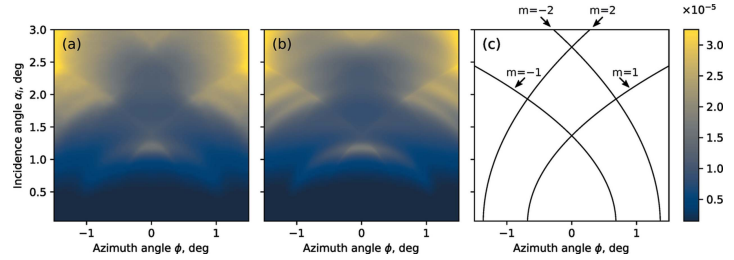
\includegraphics[width=\textwidth]{figures/resonant_maps.png}
    \caption{Двумерные угловые карты флуоресценции $(\phi, \alpha_i)$ и наложенные аналитические резонансные линии Рэлея для порядков $m = \pm 1, \pm 2$ согласно уравнению (\ref{eq:rayleigh_lines_p}).}
    \label{fig:resonant_maps_p}
\end{figure}

\newpage
\section*{Заключение}
\addcontentsline{toc}{section}{Заключение}

В настоящей работе построен строгий математический аппарат метода связанных волн (RCWA) и полуаналитического расчета выхода рентгеновской флуоресценции (GIXRF) для $p$ ($\pi$) поляризации излучения:

\begin{enumerate}
    \item Доказана необходимость применения правил факторизации Ли (Li, 1996) для корректного описания разрыва нормальной компоненты поля $E_x$ на вертикальных стенках нанорешеток. Построена устойчивая матрица взаимодействия $A = Z^{-1} (K^2 I - K_x [\varepsilon]^{-1} K_x)$ с привлечением двух взаимно обратных тёплицевых матриц $[\varepsilon]$ и $Z = [1/\varepsilon]$.
    \item Сформулированы точные граничные условия сшивки тангенциальных полей $H_y$ и $E_x \propto \frac{1}{\varepsilon} \frac{\partial H_y}{\partial z}$, устранена экспоненциальная неустойчивость традиционного TMM и получена численно стабильная глобальная СЛАУ $4D \times 4D$ и редуцированная СЛАУ $2D \times 2D$.
    \item Впервые в замкнутом матричном виде выведена обобщенная формула Николаева для выхода флуоресценции в $p$-поляризации:
    \begin{equation*}
        Y^{(p)}(\alpha_i) = \frac{1}{K^2 |\varepsilon_1|^2} \mathbf{1}^T \left\{ U \odot \big( E W^{(x)} E^H \big) + (\mathcal{K}_x U \mathcal{K}_x) \odot \big( E W E^H \big) \right\} \mathbf{1},
    \end{equation*}
    позволяющая вычислять полный флуоресцентный выход от обеих компонент поля $(E_x, E_z)$ строго аналитически менее чем за 0.5 миллисекунды.
    \item Проанализированы кинематические и динамические особенности двумерных карт $(\phi, \alpha_i)$ для $p$-поляризации, доказана инвариантность расположения линий Рэлея относительно поляризации и раскрыта физическая специфика контраста стоячих волн вблизи вертикальных границ наноструктур.
\end{enumerate}

\begin{thebibliography}{99}
\addcontentsline{toc}{section}{Список литературы}

\bibitem{nikolaev2020}
Nikolaev, K. V., et al. (2020). Characterization of ordered 3D nanostructures using grazing-incidence X-ray fluorescence and dynamic diffraction theory: a semi-analytical approach. \textit{Journal of Synchrotron Radiation}, 27(4), 1--10.

\bibitem{soltwisch2018}
Soltwisch, V., Hönicke, P., Kayser, Y., Eilbracht, J., Probst, J., Scholze, F., \& Beckhoff, B. (2018). Reference-free grazing incidence X-ray fluorescence on periodic nanostructures. \textit{Nanoscale}, 10(13), 6177--6185.

\bibitem{li1996}
Li, L. (1996). Use of Fourier series in the analysis of discontinuous periodic structures. \textit{Journal of the Optical Society of America A}, 13(9), 1870--1876.

\bibitem{moharam1995}
Moharam, M. G., Pommet, D. A., Grann, E. B., \& Gaylord, T. K. (1995). Stable implementation of the rigorous coupled-wave analysis for surface-relief gratings: enhanced transmittance matrix approach. \textit{Journal of the Optical Society of America A}, 12(5), 1077--1086.

\bibitem{hench_strakos}
Hench, J. J., \& Strakoš, Z. (2008). The RCWA method — a case study with open questions and perspectives of algebraic computations. \textit{Technical Report}, Academy of Sciences of the Czech Republic.

\bibitem{sherman1955}
Sherman, J. (1955). The theoretical derivation of fluorescent X-ray intensities from mixtures. \textit{Spectrochimica Acta}, 7, 283--306.

\bibitem{mikulik_rcwa}
Mikulík, P., \& Baumbach, T. (1999). X-ray grazing-incidence diffraction from laterally structured surfaces. \textit{Physical Review B}, 59(11), 7632--7643.

\end{thebibliography}

\end{document}
